\section*{Appendix}

\section{Question-Evidence Similarity Demonstration}
\label{sec:appndx1}

In this section, we further interpret the outcome of our contrastive loss.

We apply PCA over the relevant normalized token representations of the validation data of HotpotQA (i.e., the question and answers representations in Fig.~\ref{fig:model}), and depicted them in~\ref{fig:pca}. The projected representations of the correct and wrong answers are equally distributed at the beginning of the training (left figure). After several epochs when the model converged (right figure), the answer representations' manifold got closer to the questions' representations (in terms of radial distance). Each beam in the figure corresponds to a different question type (there are 3 in HotpotQA). The correct evidence representations (green dots) are the closest among the whole answer representations, confirming that our additional contrastive loss term generalizes and maximizes the question-evidence similarity. 


\section{Datasets and Finetuning Details}
\label{sec:appndx2}
In this section, we provide details, regrading finetuning and hyper-parameter configuration, over the benchmarks we used during our experiments.

\subsection{QAsper}
\label{subsec:qasper}
Since some of the questions included in QAsper are not answerable, we apply our contrastive loss only over examples that are answerable and contain at least one evidence sentence. 

We train all models using the Adam optimizer~\citep{kingma2014adam} and a triangular learning rate scheduler \cite{howard2018universal} with 10\% warmup. To determine number of epochs, peak learning rate, and batch size, we performed manual hyperparameter search on a subset of the training data. We searched over \{1, 3, 5\} epochs with learning rates \{$1e^{-5}$, $3e^{-5}$, $5e^{-5}$, $9e^{-5}$\}, and found that smaller batch sizes generally work better than larger ones. Our final configuration was 10 epochs, peak learning rate of $5e^{-5}$, and batch size of 2, which we used for all reported experimental settings.  When handling full text, we use gradient checkpointing~\cite{gradckpt} to reduce memory consumption. We run our experiments on a single RTX 8000 GPU, and each experiment takes 30--60 minutes per epoch. 


\subsection{HotpotQA}
\label{subsec:hotpotqa}
We used the HotpotQA-distractor dataset~\cite{yang-etal-2018-hotpotqa}. Each example in the dataset is includes a question and 10 paragraphs from different documents, extracted from Wikipedia. Two gold paragraphs include the relevant information for properly answering the question, mixed and shuffled with eight distractor paragraphs (for the full dataset statistics, see~\citet{yang-etal-2018-hotpotqa}). There are two goals for this task: detecting the supporting facts, i.e., evidence sentences, as well as extraction of the correct answer span. 

For preparing the data for training and evaluation, we follow the same finetuning scheme of the CDLM~\cite{caciularu-etal-2021-cdlm-cross} and the Longformer~\cite{longformer}; For each example, we concatenate the question and all the 10 paragraphs in one long context. We particularly use the following input format with special tokens and our document separators: ``\texttt{[CLS] [q] question [/q] $\langle$\texttt{doc-s}$\rangle$$\langle$t$\rangle$ $\texttt{title}_{\texttt{1}}$ $\langle$/t$\rangle$} \texttt{$\langle$s$\rangle$} $\texttt{sent}_{\texttt{1,1}}$ \texttt{$\langle$/s$\rangle$} \texttt{$\langle$s$\rangle$} $\texttt{sent}_{\texttt{1,2}}$ \texttt{$\langle$/s$\rangle$} $\langle$\texttt{/doc-s}$\rangle$ \texttt{...} \texttt{$\langle$t$\rangle$ $\langle$\texttt{doc-s}$\rangle$ $\texttt{title}_{\texttt{2}}$ $\langle$/t$\rangle$ }  $\texttt{sent}_{\texttt{2,1}}$ \texttt{$\langle$/s$\rangle$} \texttt{$\langle$s$\rangle$} $\texttt{sent}_{\texttt{2,2}}$ \texttt{$\langle$/s$\rangle$} \texttt{$\langle$s$\rangle$} \texttt{...}'' where \texttt{[q]}, \texttt{[/q]}, $\langle$\texttt{t}$\rangle$, $\langle$\texttt{/t}$\rangle$, \texttt{$\langle$s$\rangle$}, \texttt{$\langle$/s$\rangle$}, \texttt{[p]} are special tokens representing, question start and end, paragraph title start and end, and sentence start and end, respectively. The new special tokens were added to the models vocabulary and randomly initialized before task finetuning. We use global attention to question tokens, paragraph title start tokens as well as sentence tokens. 
The model's structure is taken from ~\citet{longformer}.

As in~\citet{longformer,caciularu-etal-2021-cdlm-cross}, we finetune our models for 5 epochs, using a batch size of 32, learning rate of $1e^{-4}$, 100 warmup steps. Finetuning on our models took $\sim$6 hours per epoch, using four 48GB RTX8000 GPUs for finetuning our models. For generating the CDLM-large results, we pretrined our version using the code from \url{https://github.com/aviclu/CDLM/tree/main/pretraining}.


\begin{figure*}
\centering
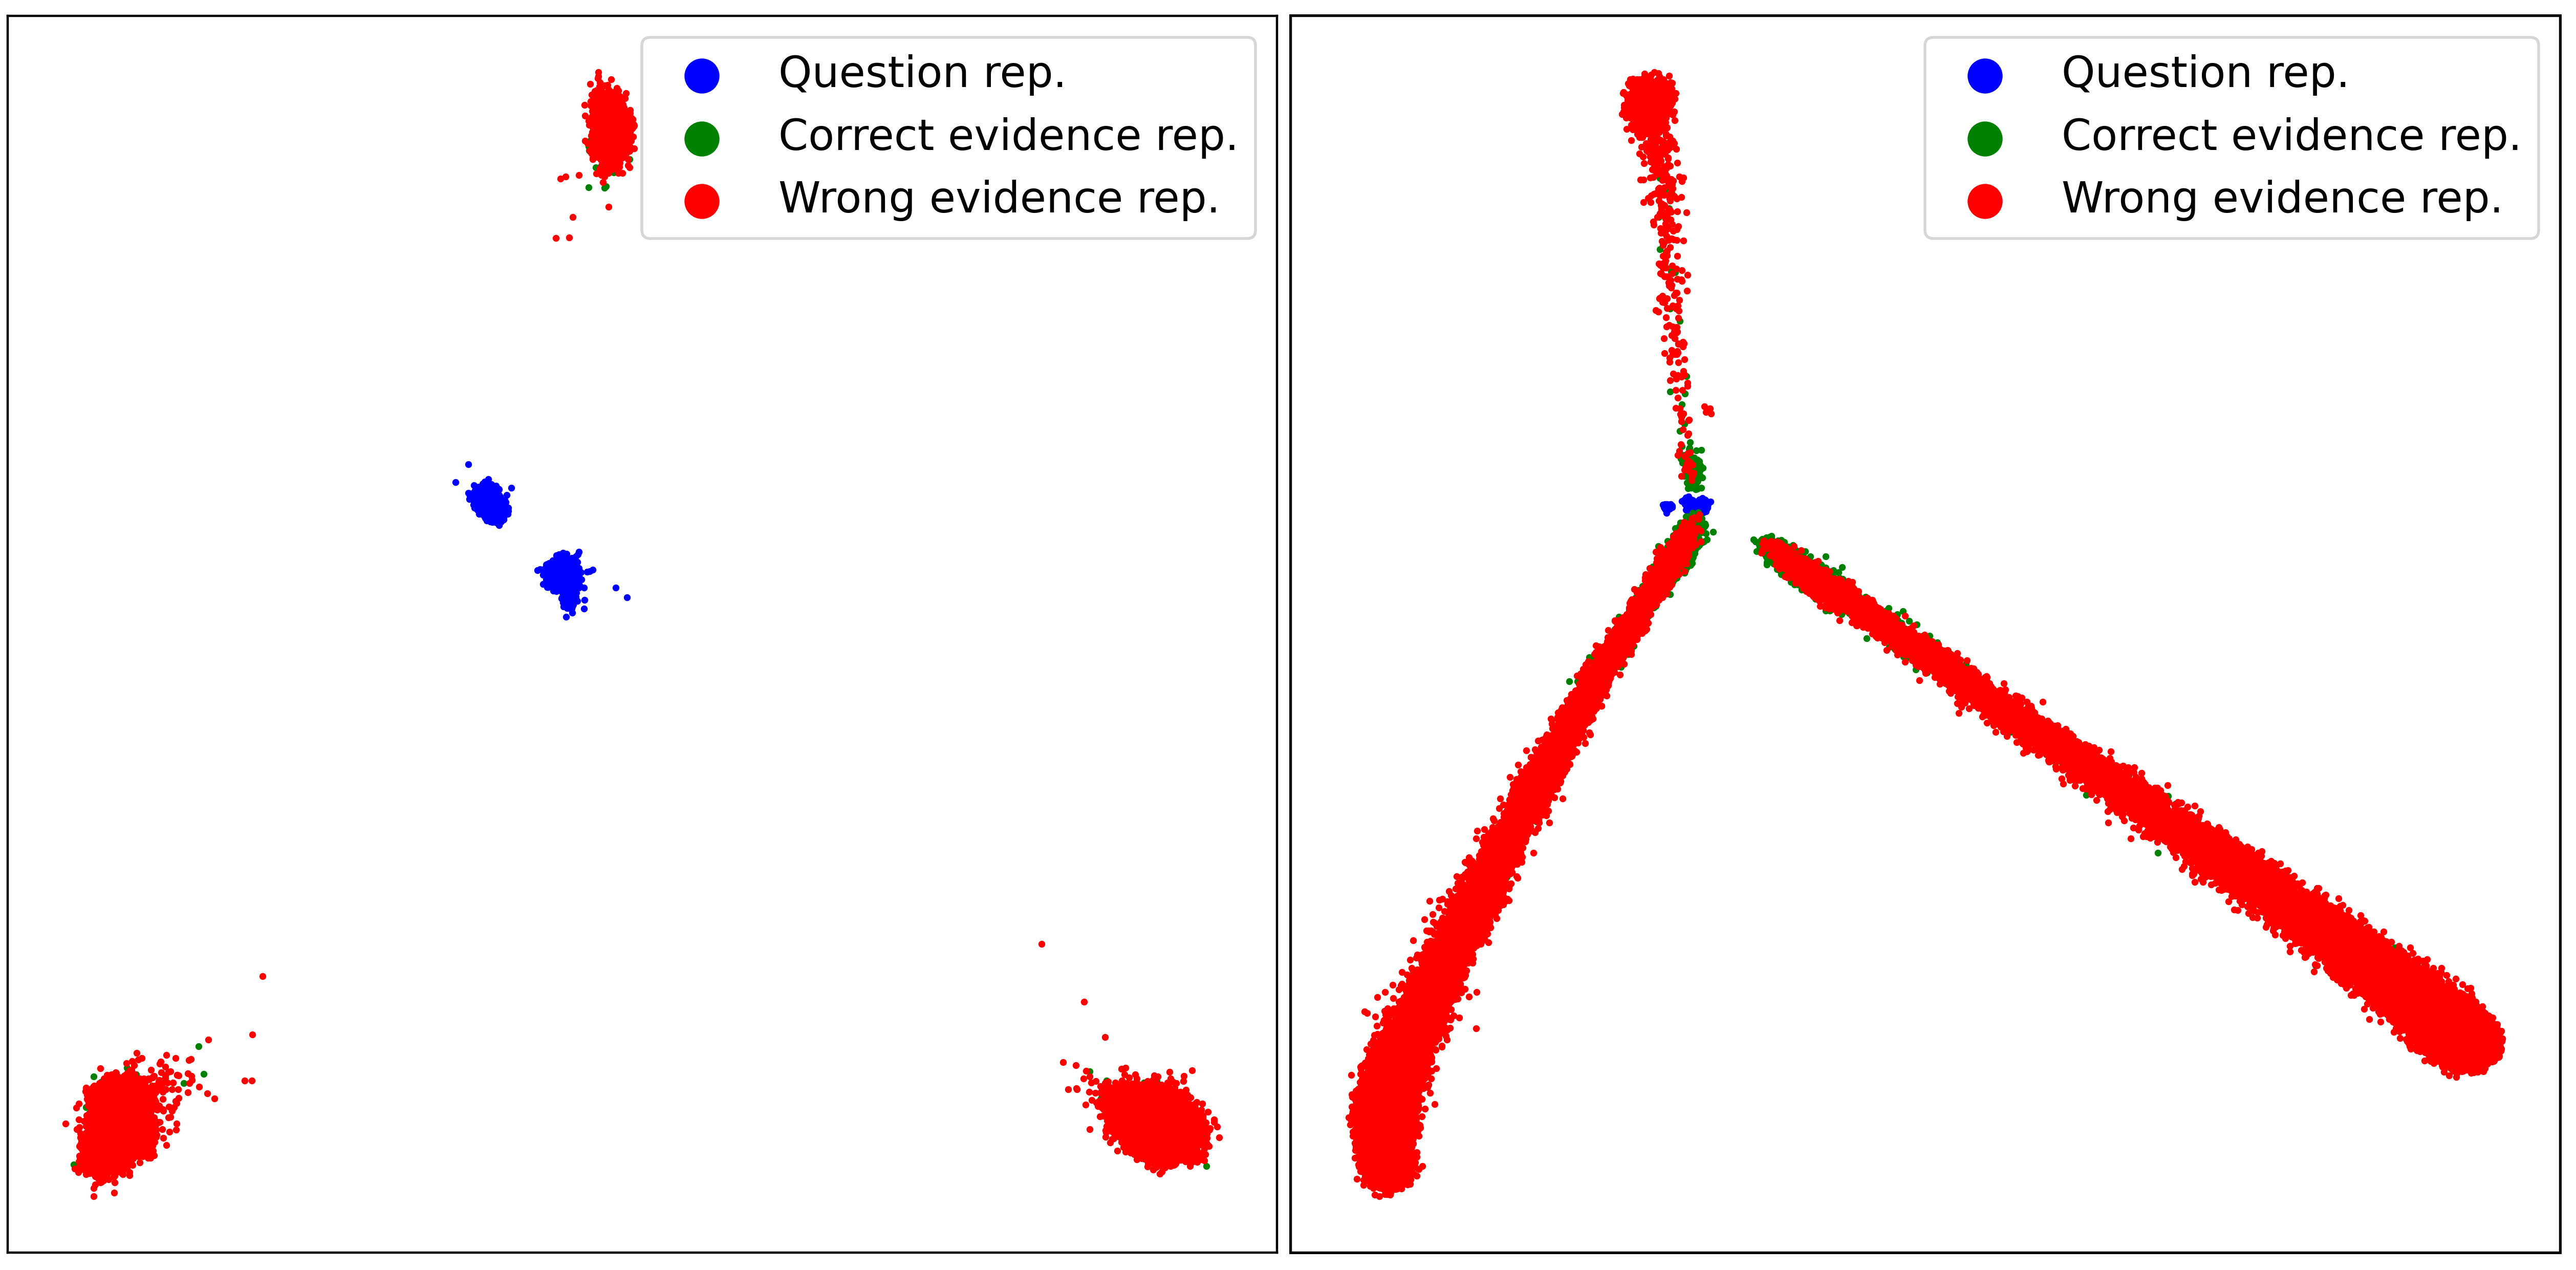
\includegraphics[width=.98\linewidth]{figures/pca_figures_3.png}
  \caption{PCA plots of the learned question and answer token embeddings on the HotpotQA validation set, comparing early training epochs results (left) and results after model convergence (right). The wrong evidence representations correspond to both wrong evidences, or correct evidences using the wrong question type projections (our soft negatives).}
  \label{fig:pca}
\end{figure*}


\section{Contrastive Loss Details}
\label{sec:contrastive}
In this section, we provide the details for reproducing our contrastive term, which is relevant for both QAsper and HotpotQA.

We searched over $d\times\{d,\frac{d}{2},\frac{d}{4},\frac{d}{8}\}$ to determine the linear projections' dimensions, where $d$ is the model's hidden layer representation dimension (it depends on the size of the model). In order to determine the temperature hyperparameter $\tau$, we searched over $\{0.2,0.4,0.6,0.8,1.0\}$ per question type (if applicable). We also applied dropout with a rate of ${p=0.1}$ over the linear projections, which consistently improved the results over all the benchmarks. Finally, we searched for the best performing $\lambda$ hyperparameter over the values of $\{0.2,0.4,0.6,0.8,1.0\}$.

